\documentclass[12pt]{report}
\usepackage[utf8]{inputenc}
\usepackage[russian]{babel}
%\usepackage[14pt]{extsizes}
\usepackage{listings}
\usepackage{graphicx}
\usepackage{amsmath,amsfonts,amssymb,amsthm,mathtools} 
\usepackage{pgfplots}
\usepackage{filecontents}
\usepackage{indentfirst}
\usepackage{eucal}
\usepackage{amsmath}
\usepackage{enumitem}
\frenchspacing

\usepackage{indentfirst} % Красная строка


%\usetikzlibrary{datavisualization}
%\usetikzlibrary{datavisualization.formats.functions}

\usepackage{amsmath}




% Для листинга кода:
\lstset{ %
language=haskell,                 % выбор языка для подсветки (здесь это С)
basicstyle=\small\sffamily, % размер и начертание шрифта для подсветки кода
numbers=left,               % где поставить нумерацию строк (слева\справа)
numberstyle=\tiny,           % размер шрифта для номеров строк
stepnumber=1,                   % размер шага между двумя номерами строк
numbersep=5pt,                % как далеко отстоят номера строк от подсвечиваемого кода
showspaces=false,            % показывать или нет пробелы специальными отступами
showstringspaces=false,      % показывать или нет пробелы в строках
showtabs=false,             % показывать или нет табуляцию в строках
frame=single,              % рисовать рамку вокруг кода
tabsize=2,                 % размер табуляции по умолчанию равен 2 пробелам
captionpos=t,              % позиция заголовка вверху [t] или внизу [b] 
breaklines=true,           % автоматически переносить строки (да\нет)
breakatwhitespace=false, % переносить строки только если есть пробел
escapeinside={\#*}{*)}   % если нужно добавить комментарии в коде
}

\usepackage[left=2cm,right=2cm, top=2cm,bottom=2cm,bindingoffset=0cm]{geometry}
% Для измененных титулов глав:
\usepackage{titlesec, blindtext, color} % подключаем нужные пакеты
\definecolor{gray75}{gray}{0.75} % определяем цвет
\newcommand{\hsp}{\hspace{20pt}} % длина линии в 20pt
% titleformat определяет стиль
\titleformat{\chapter}[hang]{\Huge\bfseries}{\thechapter\hsp\textcolor{gray75}{|}\hsp}{0pt}{\Huge\bfseries}


% plot
\usepackage{pgfplots}
\usepackage{filecontents}
\usetikzlibrary{datavisualization}
\usetikzlibrary{datavisualization.formats.functions}
\RequirePackage[
  style=gost-numeric,
  language=auto,
  autolang=other,
  sorting=none,
]{biblatex}

\addbibresource{bib.bib}
\begin{document}
%\def\chaptername{} % убирает "Глава"
\thispagestyle{empty}
\begin{titlepage}
	\noindent \begin{minipage}{0.15\textwidth}
	
\includegraphics[width=\linewidth]{b_logo}
	\end{minipage}
	\noindent\begin{minipage}{0.9\textwidth}\centering
		\textbf{Министерство науки и высшего образования Российской Федерации}\\
		\textbf{Федеральное государственное бюджетное образовательное учреждение высшего образования}\\
		\textbf{~~~«Московский государственный технический университет имени Н.Э.~Баумана}\\
		\textbf{(национальный исследовательский университет)»}\\
		\textbf{(МГТУ им. Н.Э.~Баумана)}
	\end{minipage}
	
	\noindent\rule{18cm}{3pt}
	\newline\newline
	\noindent ФАКУЛЬТЕТ $\underline{\text{«Информатика и системы управления»}}$ \newline\newline
	\noindent КАФЕДРА $\underline{\text{«Программное обеспечение ЭВМ и информационные технологии»}}$\newline\newline\newline\newline\newline
	
	
	\begin{center}
		\noindent\begin{minipage}{1.3\textwidth}\centering
			\Large\textbf{  Отчёт по лабораторным работам №3 по дисциплине}\newline
			\textbf{ "Методы машинного обучения"}\newline\newline
		\end{minipage}
	\end{center}
	
	\noindent\textbf{Тема} $\underline{\text{Проверка гипотезы о математическом ожидании - Две выборки}}$\newline\newline
	\noindent\textbf{Студент} $\underline{\text{Варламова Е. А.}}$\newline\newline
	\noindent\textbf{Группа} $\underline{\text{ИУ7-23М}}$\newline\newline
	\noindent\textbf{Оценка (баллы)} $\underline{\text{~~~~~~~~~~~~~~~~~~~~~~~~~~~}}$\newline\newline
	\noindent\textbf{Преподаватели} $\underline{\text{Солодовников Владимир Игоревич}}$\newline\newline\newline
	
	\begin{center}
		\vfill
		Москва~---~\the\year
		~г.
	\end{center}
\end{titlepage}
\large
\setcounter{page}{2}
\def\contentsname{СОДЕРЖАНИЕ}
\renewcommand{\contentsname}{СОДЕРЖАНИЕ}
\tableofcontents
\renewcommand\labelitemi{---}
\newpage
\chapter{Теоретическая часть}

Статистическая гипотеза -- гипотеза о виде распределения и свойствах случайной величины, которые можно подтвердить или опровергнуть применением статистических методов к данным выборки. Нулевая гипотеза -- принимаемое по умолчанию предположение о том, что не существует связи между двумя наблюдаемыми событиями. Нулевая гипотеза H0 считается верной, пока нельзя доказать обратное. В случае, если нулевая гипотеза отвергается, принимается альтернативная.

Проверка статистических гипотез является важным инструментом в области статистики и исследований, она позволяет делать выводы о наличии или отсутствии статистически значимых различий между наборами данных и принимать обоснованные решения на основе этих данных.

Целью данной лабораторной работы является применение методики проверки статистических гипотез при исследовании двух выборок.

Для этого необходимо решить следующие задачи:
\begin{itemize}
    \item формализовать задачу;
    \item описать методику проверки статистических гиптоез;
    \item привести особенности реализации ПО, решающего поставленную задачу;
    \item провести исследование зависимости изменения значений статистики критерия и $P-value$ для всех итераций проверки гипотезы при изменяющемся математическом ожидании одной из выборок и при изменении размеров выборки.
\end{itemize}

\section{Постановка задачи}
Сгенерировать две независимые выборки $x_1,…,x_n$ и $y_1,…,y_m$ с нормальным законом распределения и с параметрами  $(a_1,\sigma_1^2 )$ и $(a_2,\sigma_2^2 )$  соответствено. Изначально $a_1= a_2$ и $\sigma_1^2=\sigma_2^2$, число элементов $n=m=30$. Для полученных выборок предполагаем, что обе дисперсии неизвестны, но они равны между собой. 
\begin{enumerate}
    \item Осуществить проверку гипотезы $H_0$ о соответствии выборок нормальному закону распределения.
    \item Осуществить проверку гипотезы $H_0:a_1= a_2$ против альтернативы $H_1:a_1 \neq a_2$.
    \item Производить сдвиг вправо математического ожидания второй выборки $a_2$ на величину $\delta=0.01 (a_2=a_2+∆)$ и осуществлять проверку гипотезы $H_0:a_1= a_2$ до тех пор, пока гипотеза $H_0$ не будет отвергнута. 
    \item Для второй выборки назначить $a_2$ равным середине пройденного отрезка из пункта 3. Постепенно увеличивать число элементов в выборках и осуществлять проверку гипотезы $H_0:a_1= a_2$ до тех пор, пока гипотеза $H_0$ не будет отвергнута.
    \item Рассчитать 95\% доверительные интервалы для математических ожиданий двух выборок в момент, когда гипотеза $H_$0 была отвергнута в пунктах 3 и 4.
\end{enumerate}

Дополнительное представление результатов:
\begin{itemize}
    \item Вывести на экран гистограммы двух выборок; 
    \item Отобразить в виде графиков динамику изменения значений статистики критерия и $P-value$ для всех итераций проверки гипотезы из пунктов 3 и 4.

\end{itemize}
	

\section{Методика проверки статистических гипотез}
Пусть задана случайная выборка $X^m = x_1,…,x_m$ -- последовательность $m$ объектов из множества $X$. Предполагается, что на множестве $X$ существует некоторая неизвестная вероятностная мера $Ρ$.
\begin{enumerate}
    \item Формулируются нулевая $H_0$ и альтернативная $H_1$ гипотезы о распределении вероятностей на множестве $X$.
    \item Задаётся некоторая статистика (произвольная измеримая функция выборки, которая не зависит от неизвестных параметров распределения) $T:X^M  \longrightarrow R$ , для которой в условиях справедливости гипотезы $H_0$ выводится функция распределения и/или плотность распределения.
    \item Фиксируется уровень значимости -- допустимая для данной задачи вероятность того, что гипотеза на самом деле верна, но будет отвергнута процедурой проверки. Это должно быть достаточно малое число $\alpha$.
    \item На множестве допустимых значений статистики $T$ выделяется критическое множество $\omega$ наименее вероятных значений статистики $T$, такое, что $P \{T \in \omega_\alpha | H_0\} = \alpha$.
    \item Собственно статистический тест (статистический критерий) заключается в проверке условия:
    \begin{itemize}
        \item Если $T(X^m) \in \omega_\alpha$ , то делается вывод <<данные противоречат нулевой гипотезе при уровне значимости $\alpha$>>. Гипотеза отвергается.
        \item  Если $T(X^m) \in \omega_\alpha$ ,  то делается вывод <<данные не противоречат нулевой гипотезе при уровне значимости $\alpha$>>. Гипотеза принимается. 
    \end{itemize}
\end{enumerate}

\section{P-value}

P-value или p-значение -- одна из ключевых величин, используемых в статистике при тестировании гипотез. Она показывает вероятность получения наблюдаемых результатов при условии, что нулевая гипотеза верна, или вероятность ошибки в случае отклонения нулевой гипотезы.

\section{Доверительный интервал}
В математической статистике -- интервал, в пределах которого с заданной вероятностью лежат выборочные оценки статистических характеристик генеральной совокупности.

Если оценку среднего требуется связать с определённой
вероятностью, то интересующий параметр генеральной
совокупности нужно оценивать не одним числом, а интервалом.
Доверительным интервалом называют интервал, в котором с
определённой вероятностью $P$ находится значение оцениваемого показателя генеральной совокупности.

\chapter{Практическая часть}

\section{Выбор средств разработки}
В качестве языка программирования был использован язык Python, поскольку этот язык кроссплатформенный и для него разработано огромное количество библиотек и модулей, решающих разнообразные задачи. 

В частности, имеются библиотеки, включающие в себя функции проверки статистических гипотез в библиотеке \cite{bib:scipy}.

Для создания графиков была выбрана библиотека matplotlib \cite{bib:matplotlib}, доступная на языке Python, так как она предоставляет удобный интерфейс для работы с данными и их визуализации.

\section{Исследование ПО}

В листинге \ref{lst:gen1} представлен код, сдвигающий математическое ожидание одной из выборок на $\delta = 0.01$ относительно другой до тех пор, пока гипотеза $H_0$ о равенстве математических ожиданий не будет отвергнута. Кроме того, считаются доверительные интервалы для каждой из выборок после отвержения гипотезы $H_0$.

\newpage
\begin{lstlisting}[label=lst:gen1,caption=код сдвига математическое ожидание одной из выборок относительно другой]
fig, ax = plt.subplots()

delta = 0.01
interval = 0
y_s = [y]
_, p_value_equal_means = stats.ttest_ind(x, y_s[-1], equal_var=True)
means_diff = [np.mean(x) - np.mean(y_s[-1])]
values = [p_value_equal_means]
ax.hist(x, alpha=0.5, label='выборка X')
_, _, h = ax.hist(y_s[-1], alpha=0.5, label='выборка Y')

while p_value_equal_means >= 0.05:
    interval += delta
    y_s.append(np.random.normal(loc=a_2 + interval, scale=sigma_2, size=m))
    _, p_value_equal_means = stats.ttest_ind(x, y_s[-1], equal_var=True)
    values.append(p_value_equal_means)
    means_diff.append(np.mean(x) - np.mean(y_s[-1]))

def update(iternum):
    global h
    h.remove()
    plt.title("p_value = {:.3f}, interval = {}".format(values[iternum], delta * iternum))
    _, _, h = ax.hist(y_s[iternum], alpha=0.5)
    
ani = animation.FuncAnimation(fig, update, frames=len(y_s), interval=400)
ani.save('animated_plot_3.gif', writer='pillow')
print("интервал = {:.3f}, p-value = {:.3f}".format(interval, p_value_equal_means))
ci_x = stats.norm.interval(0.95, loc=np.mean(x), scale=stats.sem(x))
ci_y = stats.norm.interval(0.95, loc=np.mean(y_s[-1]), scale=stats.sem(y_s[-1]))
print("интервал выборки X = {};\nинтервал выборки Y = {}".format(ci_x, ci_y))

plt.clf()
plt.plot([i * delta for i in range(len(y_s))], means_diff, label='разница средних')
plt.plot([i * delta for i in range(len(y_s))], values, label='P-value')
plt.legend()
plt.savefig("diffs_3.png")
\end{lstlisting}


В листинге \ref{lst:gen2} представлен код, в котором увеличиается размер выборок на 200 до тех пор, пока гипотеза $H_0$ о равенстве математических ожиданий не будет отвергнута. При этом математическое ожидание выборок отличается на половину интервала, вычисленного в предыдущем пункте. Кроме того, считаются доверительные интервалы для каждой из выборок после отвержения гипотезы $H_0$.

\begin{lstlisting}[label=lst:gen2,caption=код увеличения размера выборок]
fig, ax = plt.subplots()
y_s = [y]
x_s = [x]
n_ = n
m_ = m
_, p_value_equal_means = stats.ttest_ind(x_s[-1], y_s[-1], equal_var=True)
_, _, h1 = ax.hist(x_s[-1], alpha=0.5)
_, _, h2 = ax.hist(y_s[-1], alpha=0.5)
values = [p_value_equal_means]
sizes = [n_]
means_diff = [np.mean(x) - np.mean(y)]
while p_value_equal_means >= 0.05:
    n_ += 200
    m_ += 200
    x_s.append(np.random.normal(loc=a_1, scale=sigma_1, size=n_))
    y_s.append(np.random.normal(loc=a_2 + interval / 2, scale=sigma_2, size=m_))
    _, p_value_equal_means = stats.ttest_ind(x_s[-1], y_s[-1], equal_var=True)
    values.append(p_value_equal_means)
    sizes.append(n_)
    means_diff.append(np.mean(x_s[-1]) - np.mean(y_s[-1]))
def update(iternum):
    global h1
    global h2
    h1.remove()
    h2.remove()
    plt.title("p_value = {:.3f}, size = {}".format(values[iternum], sizes[iternum]))
    _, _, h1 = ax.hist(x_s[iternum], alpha=0.5)
    _, _, h2 = ax.hist(y_s[iternum], alpha=0.5)

ani = animation.FuncAnimation(fig, update, frames=len(y_s), interval=400)
ani.save('animated_plot_4.gif', writer='pillow')
ci_x = stats.norm.interval(0.95, loc=np.mean(x_s[-1]), scale=stats.sem(x_s[-1]))
ci_y = stats.norm.interval(0.95, loc=np.mean(y_s[-1]), scale=stats.sem(y_s[-1]))
print("интервал выборки X = {};\nинтервал выборки Y = {}".format(ci_x, ci_y))
plt.clf()
plt.plot(sizes, means_diff, label='разница средних')
plt.plot(sizes, values, label='P-value')
plt.legend()
plt.savefig("diffs_4.png")
\end{lstlisting}

\newpage
Были сгенерированы выборки, представленные на рисунке \ref{fig:samples}. 

\begin{figure}[h!]
  \centering
  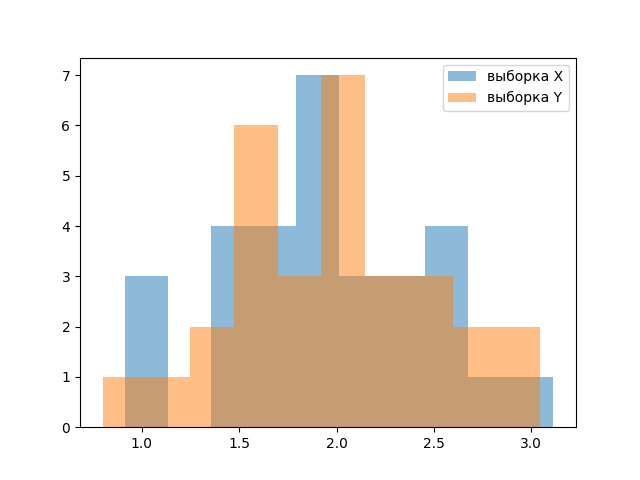
\includegraphics[width = \linewidth]{samples.png}
  \caption{}
  \label{fig:samples}
\end{figure}

Для них:
\begin{enumerate}
    \item математическое ожидание $a_1 = a_2 = 2$, дисперсия $\sigma_1 = \sigma_2 = 0.5$;
    \item размер выборок равен $30$;
    \item p-value для гипотезы о нормальном распределении для выборки $X$ составляет $0.9976$;
    \item p-value для гипотезы о нормальном распределении для выборки $Н$ составляет $0.9915$;
    \item p-value для гипотезы о равенстве математических ожиданий составляет $0.9042$;
\end{enumerate}

\newpage
Был проведен сдвиг математического ожидания выборки $Y$ с шагом $0.01$ и проверялась гипотеза о равенстве математических ожиданий. Результаты такого сдвига приведены на рисунке \ref{fig:task3}. 

\begin{figure}[h!]
  \centering
  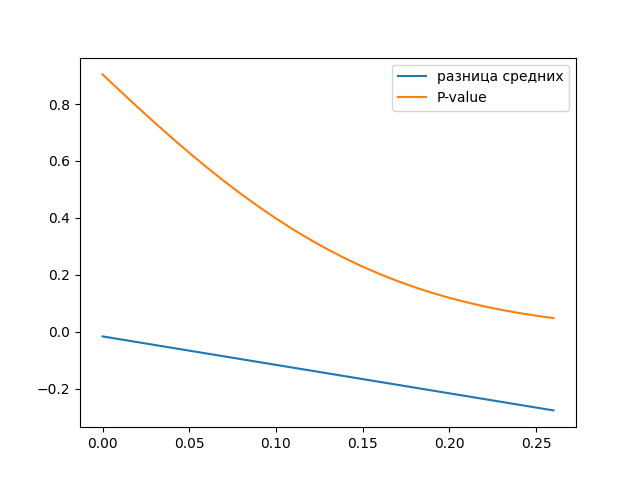
\includegraphics[width = \linewidth]{diffs_3.png}
  \caption{Заивисмость p-value от расстояния между выборками}
  \label{fig:task3}
\end{figure}

Видно, что p-value убывает с увеличением расстояния между математическими ожиданиями выборок. Когда оно достигает критического значения, равного $0.05$, гипотеза $H_0$ о равенстве отвергается.

Доверительные интервалы после отвержения гипотезы $H_0$ следующие:
\begin{itemize}
    \item интервал выборки $X = (1.76, 2.14)$;
    \item интервал выборки $Y = (2.04, 2.42)$.
\end{itemize}

\newpage

Далее был увеличен размер выборок на 200 до тех пор, пока гипотеза $H0$ о равенстве математических ожиданий не будет отвергнута. При этом математическое ожидание выборок отличается на половину интервала, вычисленного в предыдущем пункте.  Результаты приведены на рисунке \ref{fig:task4}. 

\begin{figure}[h!]
  \centering
  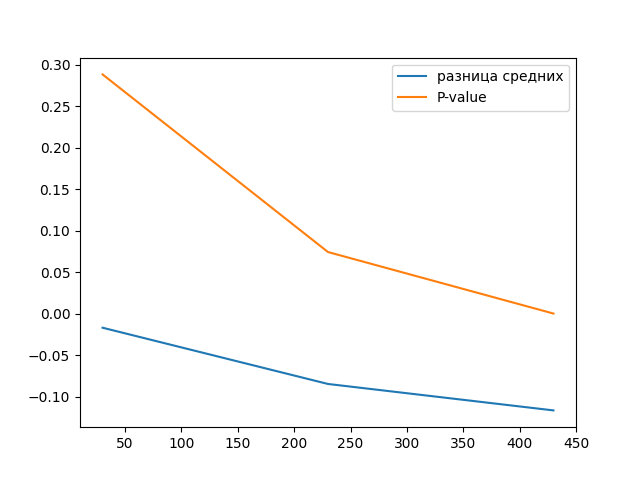
\includegraphics[width = \linewidth]{diffs_4.png}
  \caption{Увеличение размера выборок}
  \label{fig:task4}
\end{figure}

Видно, что p-value убывает с увеличением размера выборок. Когда оно достигает критического значения, равного $0.05$, гипотеза $H_0$ о равенстве отвергается.

Доверительные интервалы после отвержения гипотезы $H_0$ следующие:
\begin{itemize}
    \item интервал выборки $X = (1.96, 2.05)$;
    \item интервал выборки $Y = (2.07, 2.17)$.
\end{itemize}

\printbibliography[title={СПИСОК ИСПОЛЬЗОВАННЫХ\\ ИСТОЧНИКОВ}]
\addcontentsline{toc}{chapter}{СПИСОК ИСПОЛЬЗОВАННЫХ ИСТОЧНИКОВ}

\end{document}